\chapter{Digital Image Formation}
\label{ch:dif}

\begin{figure}
    \centering
    \pdftooltip{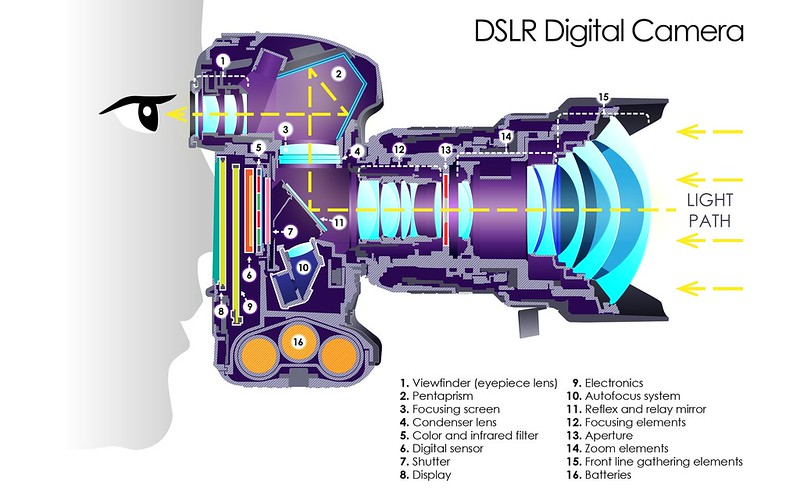
\includegraphics[width=\textwidth]{figures/light.jpg}}{Light}
    \caption{Camera and its various components \cite{cameracrosscut}.}
    \label{fig:camera}
\end{figure}

As was described in chapter \ref{ch:hvs}, digital cameras, to some extent, try to mimic the behaviour of the human eye. This attempt to mimic the human eye is achieved by combining optical elements like lenses, prisms and mirrors, mechanical elements like the shutter, and digital circuits like the imaging sensor. 

A crosscut of a typical digital single-lens reflex (DSLR) is shown in Figure \ref{fig:camera}. The camera can be seen as a light processor; each component takes in light, does some processing and passes it further for the next component to process. In the end, the photons reach the image sensor (6), where photoconversion occurs and are turned into digital units by the circuitry.

\section{Optical Systems}
\label{ss:optics}

Figure \ref{fig:optics} describes a basic ray diagram of image formation. An image of the object at a distance $d_0$ is projected to the image plane at a distance $d_i$, where the image recording material is placed. As the two rays coming from an object cross at the location of the image sensor, the resulting image is said to be in focus. The figure also shows the focal points $F$ and $F'$, which denote the location where parallel rays cross the optical axis. For an object at infinity, this is also where the object would appear in focus if we were to move the image plane from $d_i$ to $F$  \cite[159-183]{Hecht}.

Modern digital cameras, such as the one in Figure \ref{fig:camera}, consist of different lens elements of different shapes. The front elements (15) form the entrance pupil to capture as much light as possible from its surroundings and pass it to adjustable zoom elements (14), which enable the photographer to change the focal length to magnify onto subjects at various distances. The zoom elements are followed by the aperture (13) that allows us to control the amount of light reaching the sensor while keeping the rest of the elements in place \cite[159-239]{Hecht}.



\begin{figure}
\centering
\begin{tikzpicture}
    % Optical Axis
    \draw[->] (-4,0) -- (8,0) node[right] {Optical Axis};
    
    % Object
    \draw[thick] (-2,0) -- (-2,2) node[midway,left] {Object};
    
    % Lens
    \draw[thick] (0,-3) -- (0,3);
    \draw[->] (0,-3.2) -- (0,3.2) node[midway, xshift=0.5cm, yshift=0.5cm] {Lens};    
    % Focal Points
    \fill[red] (3,0) circle (2pt) node[below] {$F$};
    \fill[red] (-3,0) circle (2pt) node[below] {$F'$};
    
    % Image
    \draw[thick,blue] (4,0) -- (4,-1.5) node[midway,right] {Image};
    
    % Distance indicators
    \draw[<->, black] (-2, 2.5) -- (0, 2.5) node[midway, above] {$d_o$};
    \draw[<->, black] (0, 2.5  ) -- (4, 2.5) node[midway, above] {$d_i$};
    
    % Rays
    % Ray parallel to optical axis
    \draw[->,red] (-2,2) -- (0,2);
    \draw[->,red] (0,2) -- (3,0);
    \draw[->,red] (3,0) -- (4,-1.5);
    
    % Ray through F
    \draw[->,green] (-2,2) -- (0,0);
    \draw[->,green] (0,0) -- (4,-1.5);
    
\end{tikzpicture}

\caption{Basic image formation example.}
\label{fig:optics}
\end{figure}

Errors due to optical systems, such as colourful contours or gradual changes in brightness and colour shifts, are often attributed to how light bends when it passes from one medium to another. This phenomenon is governed by Snell's Law, which is typically presented as:

\begin{equation}
\label{eq:snell_revised}
n_1 \sin(\theta_1) = n_2 \sin(\theta_2),
\end{equation}

where $n_1$ and $n_2$ are the refractive indices of the first and second media, respectively, and $\theta_1$ and $\theta_2$ are the angles of incidence and refraction relative to the normal to the interface between the two media. However, dispersion is often omitted when discussing Snell's law, which specifies that the refractive index $n$ depends on the light's wavelength $\lambda$  \cite[108-109]{Hecht}. The refractive index can be more accurately represented as $n(\lambda)$, indicating its dependence on the wavelength. Therefore, a more precise formulation of Snell's Law that accounts for dispersion would include the wavelength dependence of the refractive indices:

\begin{equation}
\label{eq:snell_wavelength}
n_1(\lambda) \sin(\theta_1) = n_2(\lambda) \sin(\theta_2).
\end{equation}

This wavelength-dependent refractive index explains why light's different colours (wavelengths) bend at slightly different angles when passing through optical elements, leading to the optical errors observed in images. Three such errors are visualized in Figure  \ref{fig:aberration}, where light rays from a ring are first incident on a convex lens and finally reflected onto the image plane. In the topmost example, the ring is reproduced as seen in nature with no optical aberrations, as all light rays converge to the same location. In the second case, we see a noticeable blur along the edges of the ring; here, different light rays bend at slightly different angles due to dispersion, and as a result, each light ray has a different focal length, a phenomenon known as longitudinal chromatic aberration. In the third case, the light rays again converge at different locations due to dispersion, but at the same focal plane, thus this is called lateral chromatic aberration \cite[266-284]{Hecht}.

Shading is another issue arising from optics. It refers to the change in relative illumination from the centre of the captured image towards the edges, either as a decrease in luminance and/or variation in chrominance. They are respectively referred to as luminance and colour shading. Both can be characterized by taking an image under a uniform light source, known as a flat-field photograph. Uniform light can be achieved by using integrating spheres, which are typically highly uniform ($\ge$95\%) or placing a diffuser plate on top of the camera lens, spreading the incident light more evenly  \cite{ImageShading}.


Luminance shading, often referred to as vignetting, primarily results from a combination of the $cos^4(\theta)$ law, which states that there is a loss of illumination depending on the angle $\theta$, and shading related to mechanical and optical elements that might prevent some light rays from entering the sensor at particular angles. On the other hand, colour shading results from the combination of light hitting the wrong pixels due to steep angles of incidence (known as pixel cross-talk) and infrared (IR) filters, which have decreased performance when the angle of incidence increases. As such, these effects are primarily seen at the edges of the image  \cite[183-186]{Hecht}, \cite[251]{nakamura}, \cite{ImageShading}.


\begin{figure}
    \centering
    \pdftooltip{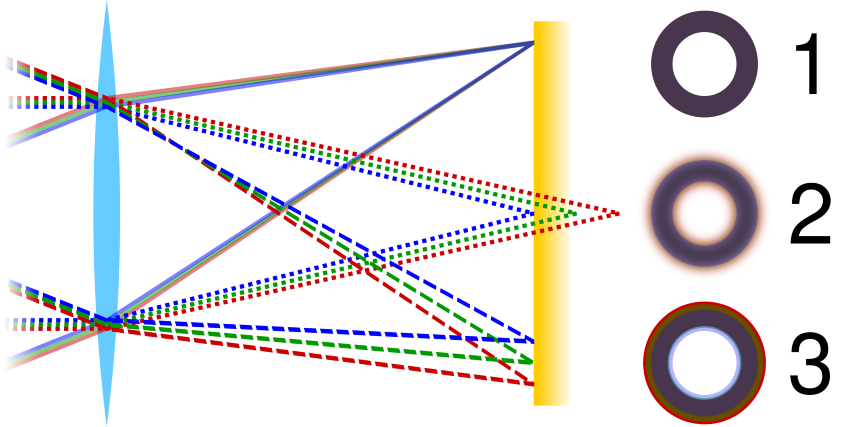
\includegraphics[scale=0.5, width=\textwidth]{figures/aberration.png}}{aberration}
    \caption{Optical aberrations \cite{aberration}. Ideal image (1), longitudinal chromatic aberration (2) and lateral chromatic aberration (3).}
    \label{fig:aberration}
\end{figure}

 
\section{Image sensors}

In the analogue era, photographic film was used to produce images, but it was slow due to the development process that had to be applied post-photography. Nowadays, the photosensitive material used is a semiconductor-based digital sensor, which converts incoming photons to electrons, resulting in an electric charge  \cite[272-274]{nakamura}. A crucial measure is then the photon energy, which is given by

\begin{equation}
\label{eq:photon}
{E_{photon}} = \frac{hc}{\lambda},
\end{equation}

where $h$ is the Planck's constant ($\approx \SI{6.626e-34}{J\cdot s}$), c is the speed of light
($\approx \SI{3e+8}{\meter\per\second}$) and $\lambda$ is the wavelength of the light. Since we have $\lambda$ in the denominator, the energy of a photon thus decreases with increasing wavelengths \cite[61-62]{Hecht} \cite[55-56]{nakamura}.

\subsection{Photoconversion}
\label{ss:photoconversion}
For a photon to convert into an electron, it must exceed the image sensor's band gap energy $E_{bg}$. However, as photons of increasing wavelengths penetrate deeper into the silicon, they begin to absorb at a lower probability. So, a photon with energy exceeding the band gap energy does not always result in an electron. A typical characteristic of an image sensor's ability to convert incident photons into electrons is its quantum efficiency (QE) \cite[77]{nakamura}. It tells us the proportion of photons that are, on average, converted into electrons and is given by the following equation: 

\begin{equation}
\label{eq:qe}
\text{QE}(\lambda) = \frac{\text{Number of electrons generated}}{\text{Number of incident photons}}
\end{equation}

The number of photons reaching a photosite depends on the exposure duration, so it is possible to compensate for quantum efficiency with more prolonged exposure durations, but generally, the better the quantum efficiency, the better the imaging sensor.

While quantum efficiency tells us how efficient the sensor is in converting photons into electrons, it does not consider the energy required to produce an electron with elementary charge $q$. From the formula in \ref{eq:photon}, it can be seen that photons with longer wavelengths have less energy, and as a consequence, it takes less energy to convert a long wavelength than a short wavelength photon into an electron. Knowing the quantum efficiency, it is then possible to compute the efficiency of photon conversion as a function of wavelength, known as the spectral responsivity (SR): 

\begin{equation}
\label{eq:sr}
\text{SR}(\lambda) =\text{QE}(\lambda) \cdot \frac{q}{E_{photon}} = \text{QE}(\lambda) \cdot \frac{q\lambda}{hc},
\end{equation}

Where QE is the quantum efficiency from \ref{eq:qe}, $E_{photon}$ is the energy of a photon for a given wavelength from \ref{eq:photon} and $q$ is the elementary charge of an electron \cite[78-79]{nakamura}.

In Figure  \ref{fig:qe}, we plot the normalized quantum efficiencies and spectral responsivities for each channel of the KAF-8300 image sensor by On Semiconductor in dashed and solid lines, respectively, in line with the formulas \ref{eq:qe} and \ref{eq:sr}, we see how, for the longer wavelengths, the spectral responsivities tend to increase relative to the corresponding quantum efficiencies. It thus takes less energy to produce a signal in the red channel than, for example, in the green channel of an image sensor.

\begin{figure}
    \centering
    \pdftooltip{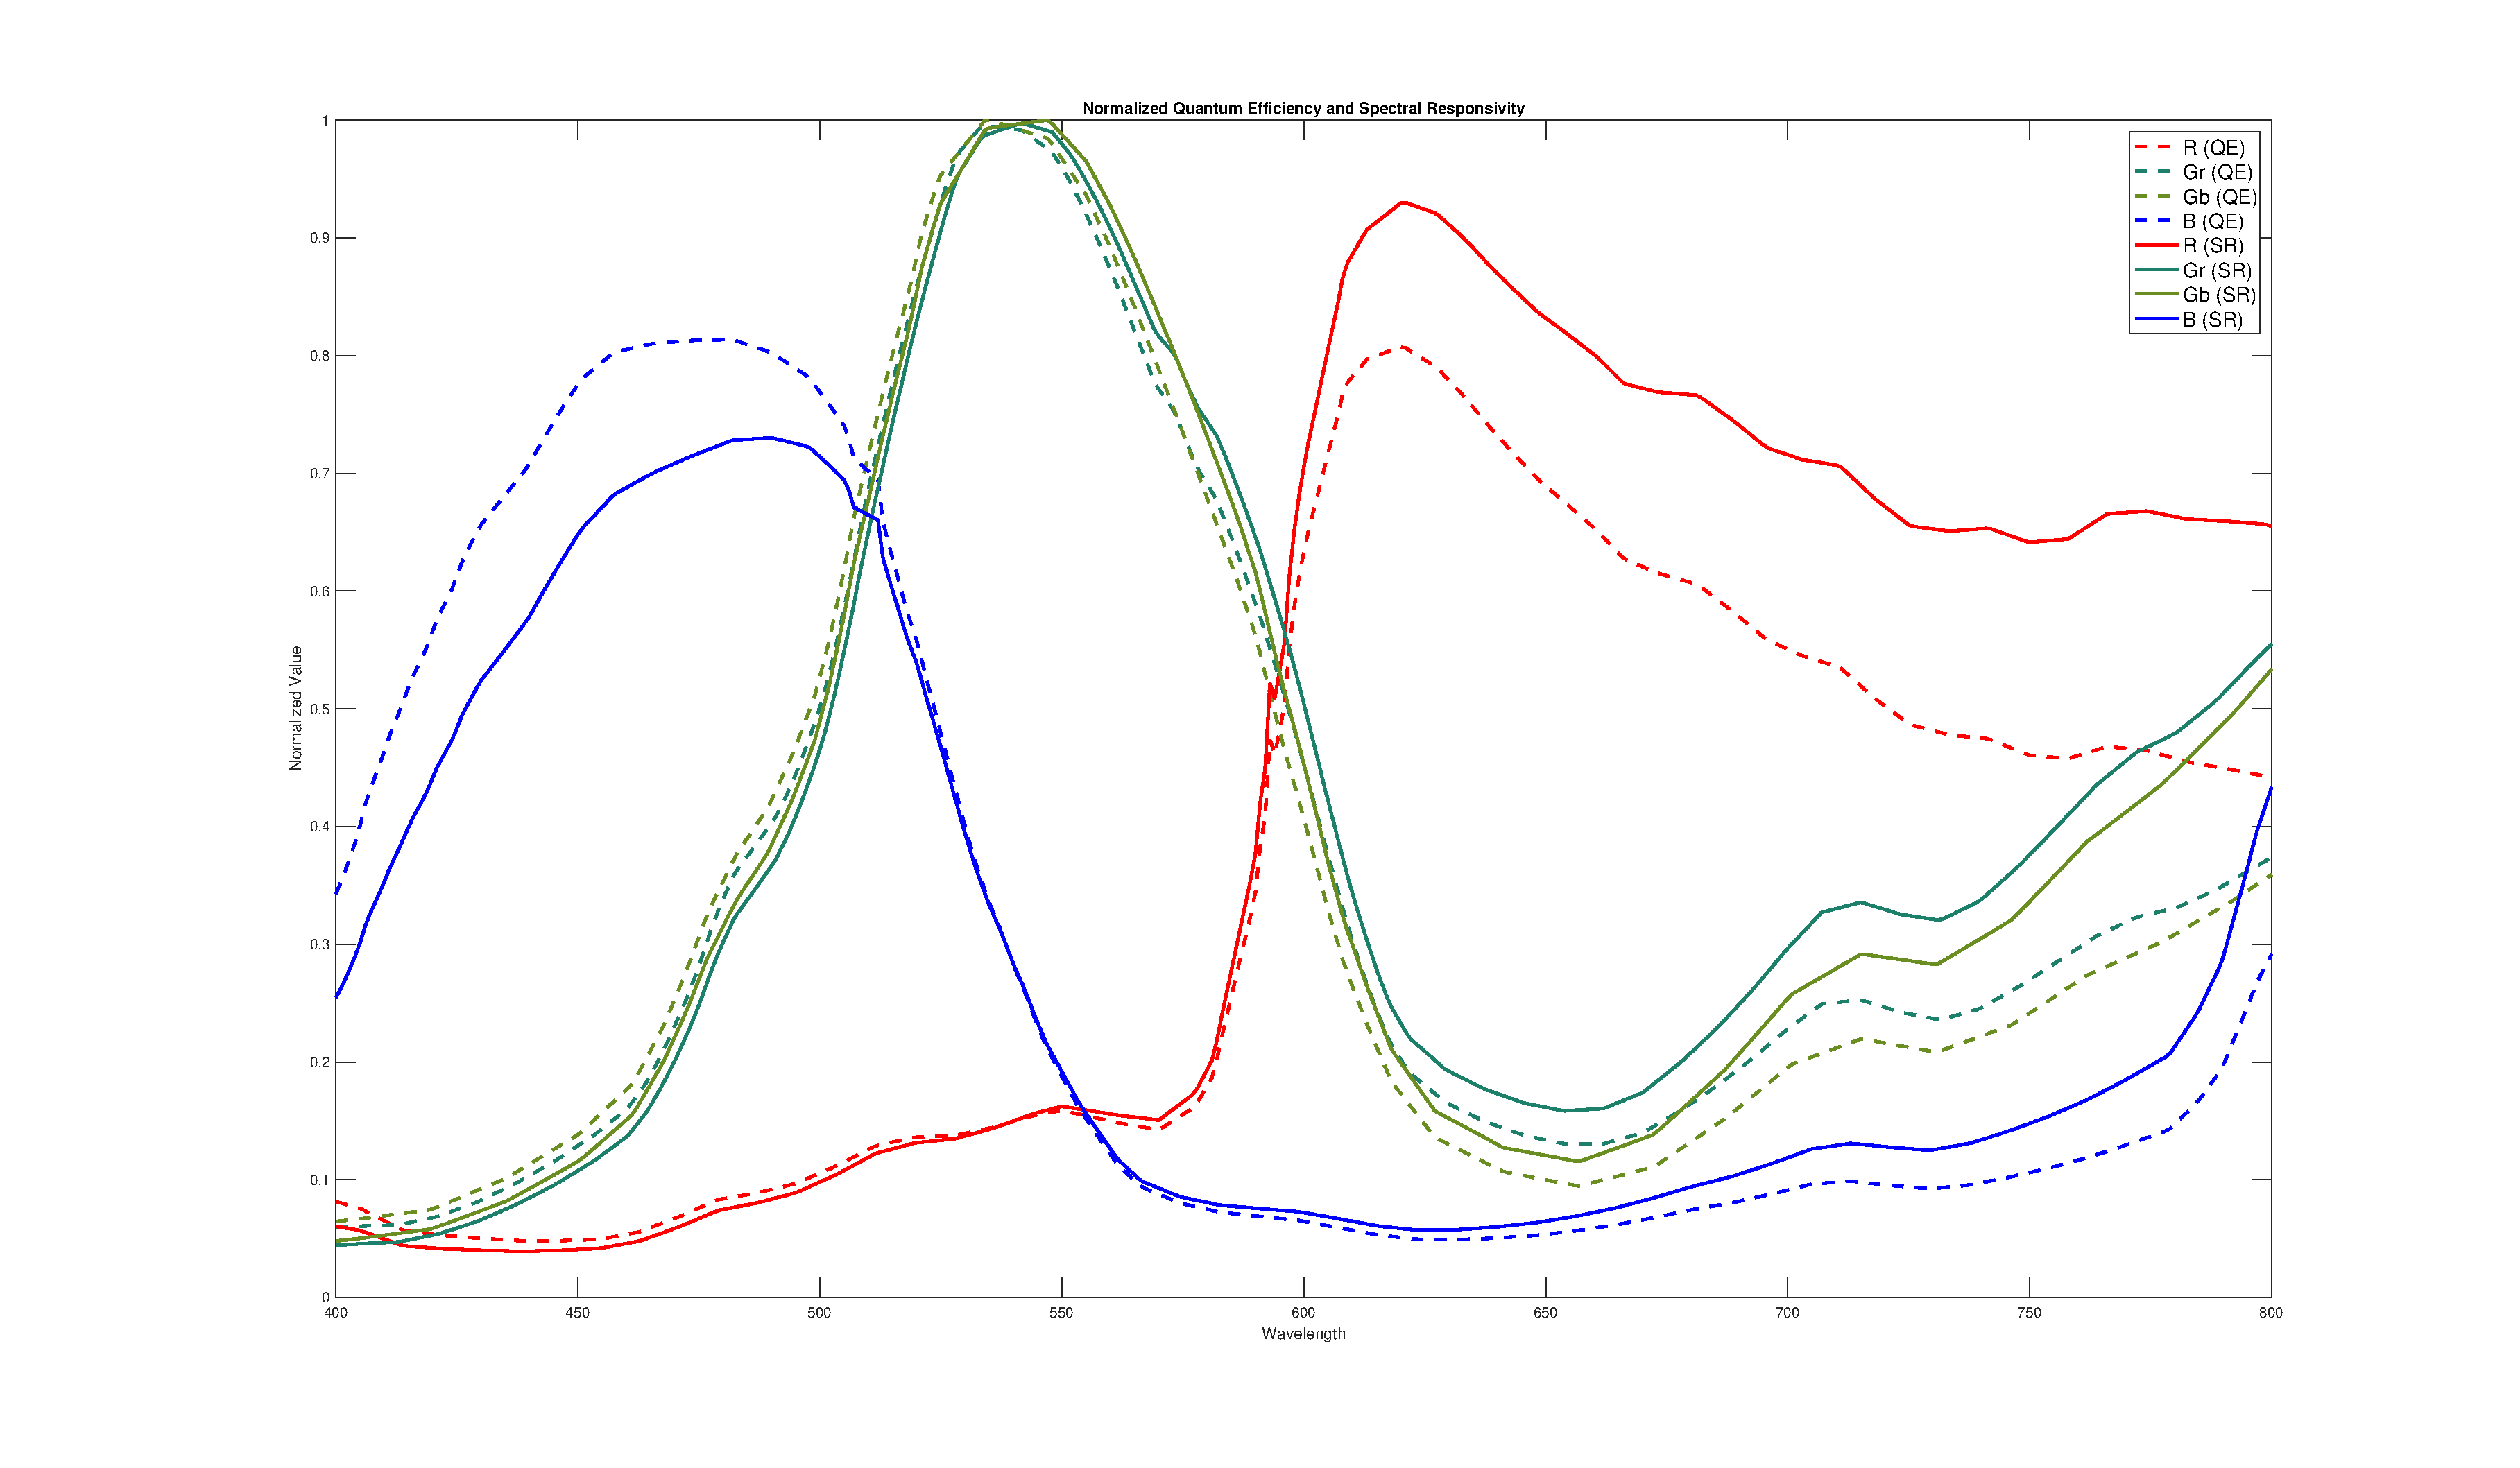
\includegraphics[width=\textwidth]{figures/normalizedqrsr.eps}}{SR}
    \caption{Normalized quantum efficiencies (dashed) and spectral sensitivities of KAF-8300 Image Sensor by OnSemi \cite{onsemi}.}
    \label{fig:qe}
\end{figure}

\subsection{Sensor types}

Currently, two dominant digital image sensor types exist:  Charge-coupled device (CCD) \\ and Complementary Metal–Oxide–Semiconductor (CMOS). Both operate similarly in \\ terms of photoconversion but differ in their internal process of converting the charge to a digital value. In both cases, colour information is achieved by placing optical filters on top of the imaging sensor, which will be discussed in \ref{ss:colour}  \cite[17]{nakamura}.

A diagram of the CCD structure can be seen in Figure \ref{fig:ccd}. The operation principle of a CCD sensor is based on having passive pixels that only collect charge and do no additional processing. When the shutter is opened, the pixels start to collect light until the shutter is closed again. Each pixel is overlaid with metal surrounded by insulating material that attracts electrons row-by-row into a serial shift register that propagates each electron into an amplifier, converting the small charge into a voltage. The movement of electrons is achieved due to their tendency to move towards a higher potential. So, by alternatively switching the voltage between adjacent pixels in a column, the electrons can be propagated downwards. The voltage is then converted to a digital value through an analog-to-digital converter (ADC)  \cite[95-139]{nakamura}, \cite[4]{Park2016}.


\begin{figure}
    \centering
    \pdftooltip{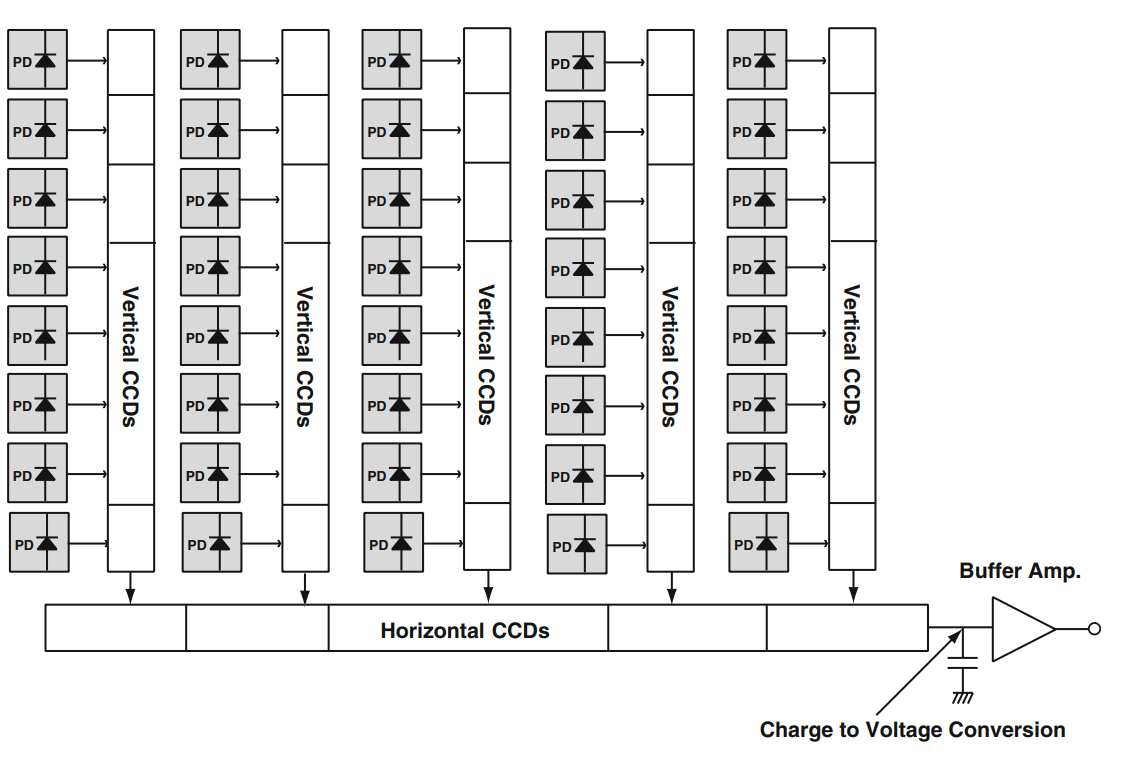
\includegraphics[width=\textwidth]{figures/ccd.png}}{CCD}
    \caption{CCD diagram. Figure copied with permission from the publisher \cite[4]{Park2016}.}
    \label{fig:ccd}
\end{figure}

 The CMOS sensor, for which the structure can be seen in Figure \ref{fig:cmos}, is more commonly used nowadays and takes an active pixel approach. An active pixel converts the charge to an analogue voltage at the photosite instead of sequentially processing each pixel through the same unit. The charges are then propagated row by row into an ADC. Since each pixel amplifies and converts to a voltage, the system can utilize parallelization efficiently. New designs might also have multiple ADCs, for example, per column, so the entire row can be converted into a digital value at once or at each photosite next to the amplifier, increasing the speed even further  \cite[144-176]{nakamura}, \cite[5]{Park2016}.

\begin{figure}
    \centering
    \pdftooltip{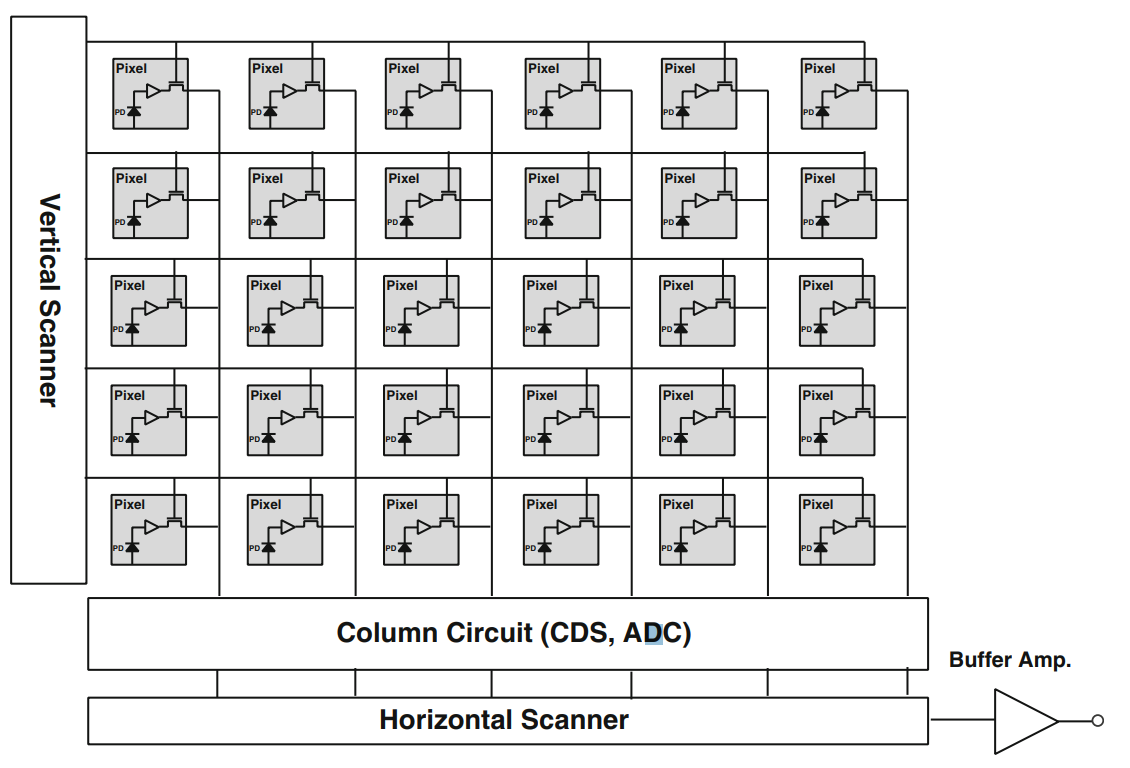
\includegraphics[width=\textwidth]{figures/cmos.png}}{CMOS}
    \caption{CMOS diagram. Figure copied with permission from the publisher \cite[5]{Park2016}.}
    \label{fig:cmos}
\end{figure}



\subsection{Pixel size}
\label{sec:fwc}

Cameras have been fitted into every mobile phone manufactured in the past decade. Since mobile phones are multi-purpose devices, the image sensors must not take up much space but still produce sharp, high-resolution images. The trick to downsizing image sensors from large digital single-lens reflex cameras (DSLRs) form factor has been to reduce the individual pixel sizes   \cite{xiao2009mobile}, \cite[308-309]{nakamura}.

The tradeoff with small pixels is that they cannot accumulate the amount of charge a large pixel would. Since a larger pixel also has a larger surface area, it can collect more photons during the exposure. A common analogy to this is to think of the different-sized pixels as buckets under a rainy sky, where each raindrop is a photon. As is shown in Figure \ref{fig:photonrain}, the result is that for different pixel sizes, the amount of collected water in proportion to the bucket size is the same for each bucket. However, as the giant bucket collects rain from a wider area, it collects more rain overall  \cite[2.27]{rowlands2020physics}. Analugous to the bucket volume, a pixel's amount of charge before saturating is known as \textbf{full-well capacity} (FWC) \cite[66]{nakamura}.

\begin{figure}
    \centering
    \pdftooltip{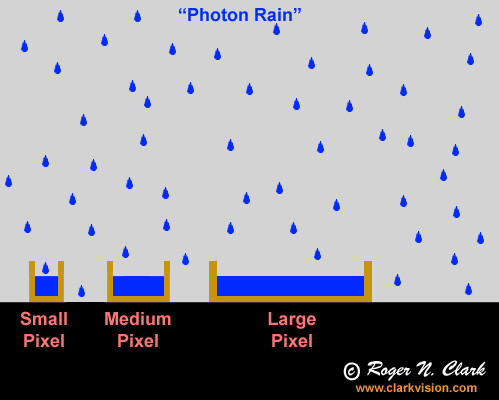
\includegraphics[scale=0.8]{figures/photon rain.png}}{PR}
    \caption{Photon rain \cite{clarkvision}.}
    \label{fig:photonrain}
\end{figure}

However, the number of photons emitted from a source per time period is not constant as expected but slightly varies. Because of their quantum nature, photons are discrete and independent of each other, making it impossible to observe fractional photon counts over any duration  \cite[61-67]{nakamura}. As such, the number of photons counted at a detector, such as an image sensor, follows a Poisson distribution:

\begin{equation}
\label{eq:poisson}
P(k; \lambda) = \frac{\lambda^k e^{-\lambda}}{k},
\end{equation}

where $\lambda$ is the mean of the distribution over a time period and $k$ is the number of realizations for a specific time period. For image sensors, the mean number of incident photons over multiple time periods (exposure times) can be taken as $\lambda$ and the number of photons for any individual period as $k$. 

For Poisson distribution, the variance is equal to the average, and so the standard deviation is the square of the mean, $\sigma = \sqrt{\lambda}$. Consequently, the SNR decreases as the average count of photons increases since the noise only grows as a square of the average signal level. This explains why noise is most prevalent when imaging in low-light conditions \cite[62, chapter. 3]{rowlands2020physics}.

\subsection{Colour Formation}
\label{ss:colour}

In the last section, we mentioned that spectral responsivity quantifies the energy required per wavelength to convert an electron into a photon. In this conversion process, the wavelength information is lost, as any photon exceeding the band gap level could have produced the electron. Image sensors are thus unable to distinguish colour and are monochromatic by nature.

The most common solution is an optical colour filter array (CFA), which forms a grid similar to the image sensor but filters light by its wavelength instead. Colour can be detected by designing the filters to allow light only in the red, green, or blue wavelength ranges. If we know the pattern of this filter, we have a rough idea of what kind of colour was incident on a specific pixel when reading the values recorded. A typical setup consists of identical blocks of 4 colour filters, a red, blue and two green filters. The reason for using twice as many green filters is that the human visual system is also more sensitive to the green wavelengths \cite[36]{Ramanath}, \cite[62-63]{nakamura}. This filter is also known as the Bayer filter after its inventor, Bruce Bayer \cite{Bayer1976}.

It is also possible to acquire colour information without a colour filter array. The most commonly known alternative, produced by Foveon, instead utilizes information about the silicon penetration depth to discriminate the colour of an incident photon \cite{lyon2002eyeing}, \cite{hubel2005foveon}. As was discussed in section \ref{ss:photoconversion}, higher wavelength photons penetrate deeper into the silicon, and thus, the colour of a photon can be read by measuring the charge generated at different depths. A diagram showing a high-level structure of a Foveon pixel is shown in Figure \ref{fig:foveon}. The main advantage of a Foveon sensor is that colour information is achieved at each pixel without demosaicking, unlike with Bayer colour filter arrays.

\begin{figure}
\centering
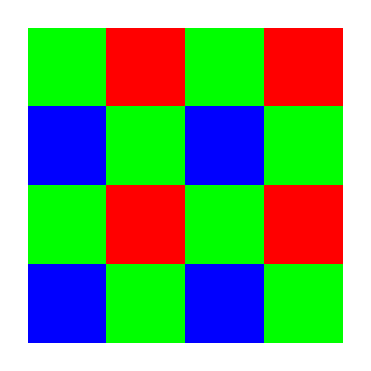
\begin{tikzpicture}

% Loop to draw the squares
\foreach \i in {0,1,2,3} {
    \foreach \j in {0,1,2,3} {
        \pgfmathtruncatemacro{\row}{mod(\i, 2)}
        \pgfmathtruncatemacro{\col}{mod(\j, 2)}
        
        % Choose color based on position
        \ifnum \row=0
            \ifnum \col=0
                \def\fillcolor{blue}
            \else
                \def\fillcolor{green}
            \fi
        \else
            \ifnum \col=0
                \def\fillcolor{green}
            \else
                \def\fillcolor{red}
            \fi
        \fi

        % Draw the square
        \fill[\fillcolor] (\i,\j) rectangle ++(1,1);
    }
}

\end{tikzpicture}
\caption{Color Filter Array.}
\label{fig:cfa}
\end{figure}

\begin{figure}
    \centering
    \pdftooltip{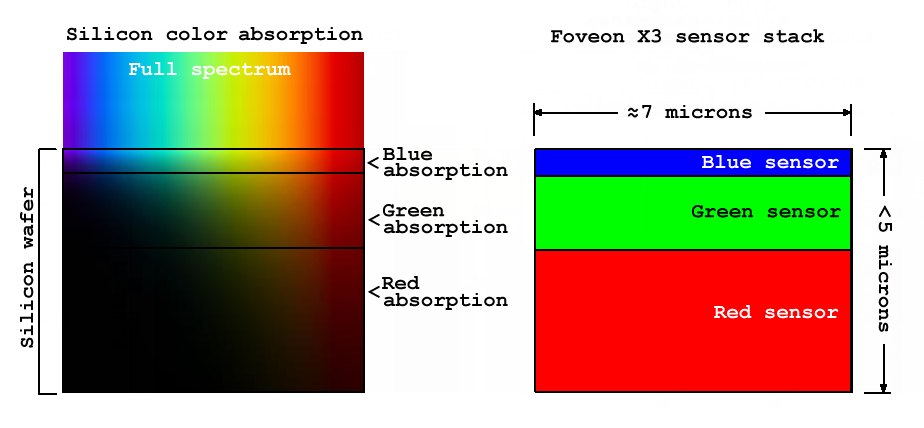
\includegraphics[width=\textwidth]{figures/foveon.png}}{Foveon}
    \caption{Colour sensing mechanism in Foveon sensors \cite{foveon}.}
    \label{fig:foveon}
\end{figure}


 The spectral sensitivities of the Nikon D5100 digital single-lens reflex camera (DSLR), measured by \citeauthor{D5100NPL}, are shown in Figure  \ref{fig:d5100}. It is apparent that since the green channel is relatively sensitive to all wavelengths, it would produce a higher response for an equal-energy (standardized as CIE E) illuminant than the other channels. Similarly, as for the human visual system, the imaging sensor computes its response to the incoming light by integrating the product of the illuminant's power spectral distribution, spectral reflectance of the object and the spectral responsivity of the sensor for a given colour over the wavelength range of interest.

\begin{figure}
    \centering
    \pdftooltip{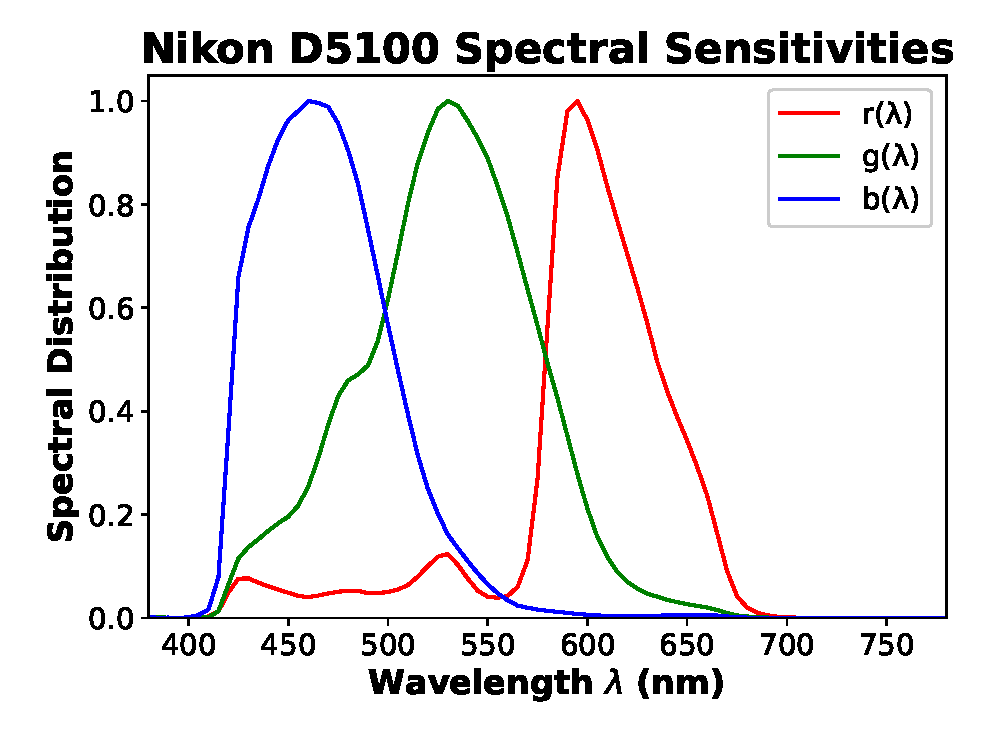
\includegraphics[width=\textwidth, scale=0.8]{figures/d5100_rgb.eps}}{nikon}
    \caption{Nikon D5100 Spectral Sensitivities  \cite{D5100NPL}.}
    \label{fig:d5100}
\end{figure}

\begin{subequations}
\begin{align}
\label{eq:sensor}
R = \int_{\lambda_{\text{min}}}^{\lambda_{\text{max}}} E(\lambda) R(\lambda) S_R(\lambda) \, d\lambda \\
G = \int_{\lambda_{\text{min}}}^{\lambda_{\text{max}}} E(\lambda) R(\lambda) S_G(\lambda) \, d\lambda \\
B = \int_{\lambda_{\text{min}}}^{\lambda_{\text{max}}} E(\lambda) R(\lambda) S_B(\lambda) \, d\lambda,
\end{align}

\end{subequations}

where $E(\lambda)$ is the spectral power distribution (SPD) of the illuminant, $R(\lambda)$ is the spectral reflectance of the imaged object and $S_T(\lambda)$ is the sensitivity of the sensor for tristimulus value $T$ (either $R$, $G$ or $B$). $\lambda_{\text{min}}$ and $\lambda_{\text{maxja }}$ are defined by the optical system, typically restricted to the visible range $\lambda_{\text{min}}$ = 380 nm and $\lambda_{\text{max}}$ = 780 nm.


\section{Image Signal Processing Pipeline}


Producing a perceptually pleasing image involves several processing steps typically executed within the camera. These steps are orchestrated by a computing unit known as the Image Signal Processor (ISP). The tasks within the ISP are divided into distinct blocks, which can operate in parallel or series, depending on the specific processing requirements \cite[91-101]{phillips2018camera}. Figure \ref{fig:dip} illustrates a typical colour image processing pipeline.

\begin{figure}
\centering
\usetikzlibrary{shapes.geometric, arrows}

\tikzstyle{startstop} = [rectangle,
minimum width=3cm, 
minimum height=1cm,
text centered, 
draw=black, 
fill=red!30]

\tikzstyle{io} = [trapezium, 
trapezium stretches=true, % A later addition
trapezium left angle=70, 
trapezium right angle=110, 
minimum width=3cm, 
minimum height=1cm, text centered, 
draw=black, fill=blue!30]

\tikzstyle{process} = [rectangle, 
minimum width=3cm, 
minimum height=1cm, 
text centered, 
text width=3cm, 
draw=black, 
fill=orange!30]

\tikzstyle{decision} = [diamond, 
minimum width=3cm, 
minimum height=1cm, 
text centered, 
draw=black, 
fill=green!30]
\tikzstyle{arrow} = [thick,->,>=stealth]

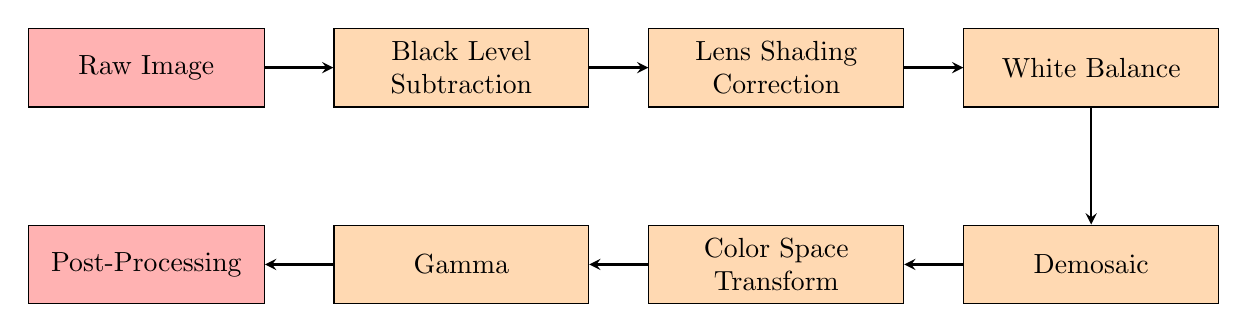
\begin{tikzpicture}[node distance=2cm]

\node (start) [startstop] {Raw Image};
\node (in1) [process, right of=start, xshift=2cm] {Black Level Subtraction};

\node (pro1) [process, right of=in1, xshift=2cm] {Lens Shading Correction};
\node (dec1) [process, right of=pro1, xshift=2cm] {White Balance};

\node (pro2a) [process, below of=dec1, yshift=-0.5cm] {Demosaic};

\node (pro2b) [process, left of=pro2a, xshift=-2cm] {Color Space Transform};
\node (pro2c) [process, left of=pro2b, xshift=-2cm] {Gamma};
\node (pro2d) [startstop, left of=pro2c, xshift=-2cm] {Post-Processing};



\draw [arrow] (start) -- (in1);
\draw [arrow] (in1) -- (pro1);
\draw [arrow] (pro1) -- (dec1);
\draw [arrow] (dec1) -- (pro2a);
\draw [arrow] (pro2a) -- (pro2b);
\draw [arrow] (pro2b) -- (pro2c);
\draw [arrow] (pro2c) -- (pro2d);

\end{tikzpicture}

\caption{Simplified colour image processing pipeline. Adapted from \cite{Ramanath}, \cite{JianpingZhou2007IPTf}.}
\label{fig:dip}
\end{figure}

Each block in the pipeline has adjustable parameters that can be fine-tuned to meet specific preferences or requirements. Image quality experts are often utilized in the industry to optimize these parameters and to perform experiments on subjective image quality, using, for example, ordinary people and their preferences \cite[29]{phillips2018camera}.


\subsection{Black Level Subtraction}

\begin{figure}
    \centering
    \pdftooltip{
\includegraphics[width=\textwidth]{figures/darkframe.jpg}}{darkframe}
    \caption{Dark frame taken on a Nikon D300, with enhanced contrast to highlight the noise \cite{darkframe}.}
    \label{fig:darkframe}
\end{figure}

Dark current is a noise source in photography, mostly prevalent at long exposures. It is also known as dark noise and can be observed by covering the camera lens entirely with a lens cap so that no light is incident on the sensor, and one would expect it not to record any voltage. However, this is wrong as the temperature around the sensor may cause electrons to be emitted, so a signal is recorded within the sensor. This type of noise can be characterized by measuring the average signal recorded under an environment where no light is incident on the sensor \cite[289]{nakamura}, \cite[63, chapter. 3]{rowlands2020physics}, \cite{Ramanath}. This image is often called a dark frame and is shown in Figure \ref{fig:darkframe}. To remove the effect of the dark noise on an image, the dark frame can then be removed from the following captured images. The process is often called Black Level Subtraction (BLS).

\subsection{Lens Shading Correction}

As was discussed in \ref{ss:optics}, lens shading results in the edges of the image having decreased brightness or variation in colour. The correction is typically performed by first characterizing the shading with a flat-field image, as was described in the same section. As this flat-field image has to be saved on the device for correction purposes, it is often downsampled before characterization into a look-up table of smaller size and interpolated at runtime \cite[251]{nakamura}, \cite{Park2016ISP}. This process is thus called Lens Shading Correction (LSC).

Luminance shading can be fixed by generating an inverse of the captured flat-field image, where the entries are the gain factors that must be applied to achieve similar brightness as in the centre of the image. \cite[286-287]{nakamura}. Depending on the optical system, the corners may sometimes be drastically darker in the flat-field image, and correcting them entirely in the digital domain would result in noisy corners. As such, the lens shading correction might not remove the shading altogether.

On the other hand, colour shading requires generating a similar correction table, but for each channel separately. Since for a uniformly illuminated image, it would be expected that the colour channels would be equal at every pixel location, the correction table is typically derived as a relative measure to some other channel's value \cite[286-287]{nakamura}. Since the green channel is typically the brightest in an image, the table is often generated by the ratio of red and blue values to the green values, $R/G$ and $B/G$.

\subsection{White Balance}
The concept of white balance (WB) in cameras, as explained in \cite[ch.~4.6]{rowlands2020physics}, is employed to replicate the phenomenon of chromatic adaptation discussed in section \ref{sec:chromaticadaptation}. WB is achieved by estimating the illuminant present in the scene and employing pre-defined multipliers to the pixel values that would equal the red, green and blue responses for an object that appears white to a human. As each illuminant might result in different proportions of red, green and blue responses for an object that appears white to a human, these multipliers are computed for a set of distinct illuminant types. This process, combined with colour correction (CC), cancels the effect of the illuminant and thus simulates the chromatic adaptation behaviour. 

The illuminant estimation algorithm primarily determines the accuracy of WB algorithms. A wrong estimation results in an improper choice of multipliers for colour correction (CC) and WB, leading to a distinct tint in the output image. Thus, the illuminant estimation process is perhaps the most important in the colour processing pipeline. For a review on illuminant estimation algorithms, we refer the reader to \cite{colourconstancy}.

Figure \ref{fig:wb} showcases the effect of applying WB. The images were simulated with Nikon D5100 spectral sensitivities \cite{D5100NPL} using scene reflectances from the dataset by \citeauthor{foster:2002} \cite{foster:2002}, under a D65 illuminant. Contrary to the figure in \ref{fig:dip}, demosaicking has been performed before white balancing. The left image has a noticeable green cast due to the spectral sensitivity imbalance between the channels. On the right side, it has been corrected by calculating the response to a Lambertian reflectance and the factors that make the channel responses even.

\begin{figure}
    \centering
    \pdftooltip{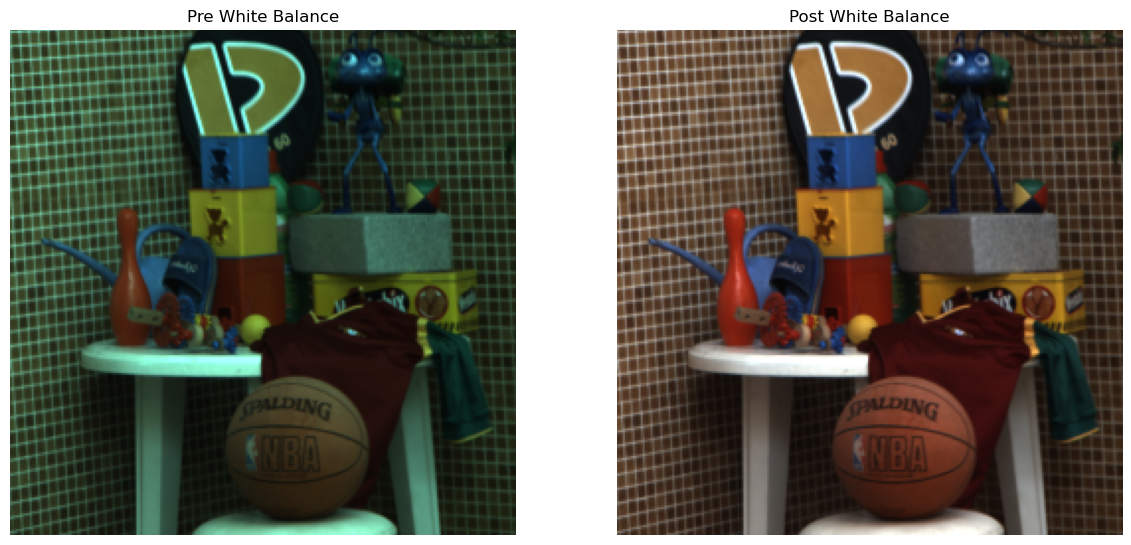
\includegraphics[width=\textwidth]{figures/wbnowb.png}}{wb}
    \caption{Scene before and after applying white balance, both with sRGB gamma applied. Image from Foster 2002 dataset \cite{foster:2002}. }
    \label{fig:wb}
\end{figure}

\subsection{Colour Filter Array Interpolation}

As discussed in Section \ref{ss:colour}, producing colour images begins with the image sensor being overlaid with a colour filter array. This array allows only light of specific wavelengths to pass through, a concept illustrated in \ref{fig:cfa}. The next step in creating a full-colour image involves a crucial process known as demosaicing.

Demosaicing employs various interpolation techniques to achieve colour accuracy. The simplest is the bilinear interpolation, based on direct interpolation methods. However, as documented in practical applications, these simple algorithms can sometimes fail, particularly at image edges \cite[46]{Ramanath}.

Acknowledging these limitations, researchers have developed more sophisticated algorithms. These advanced methods leverage cross-correlations between channels, adaptive filters, and frequency information. Such enhancements significantly improve the performance of demosaicing algorithms. Interested readers may refer to \cite{gunturk2005demosaicking} for a more detailed discussion.


\begin{figure}
    \centering
    \pdftooltip{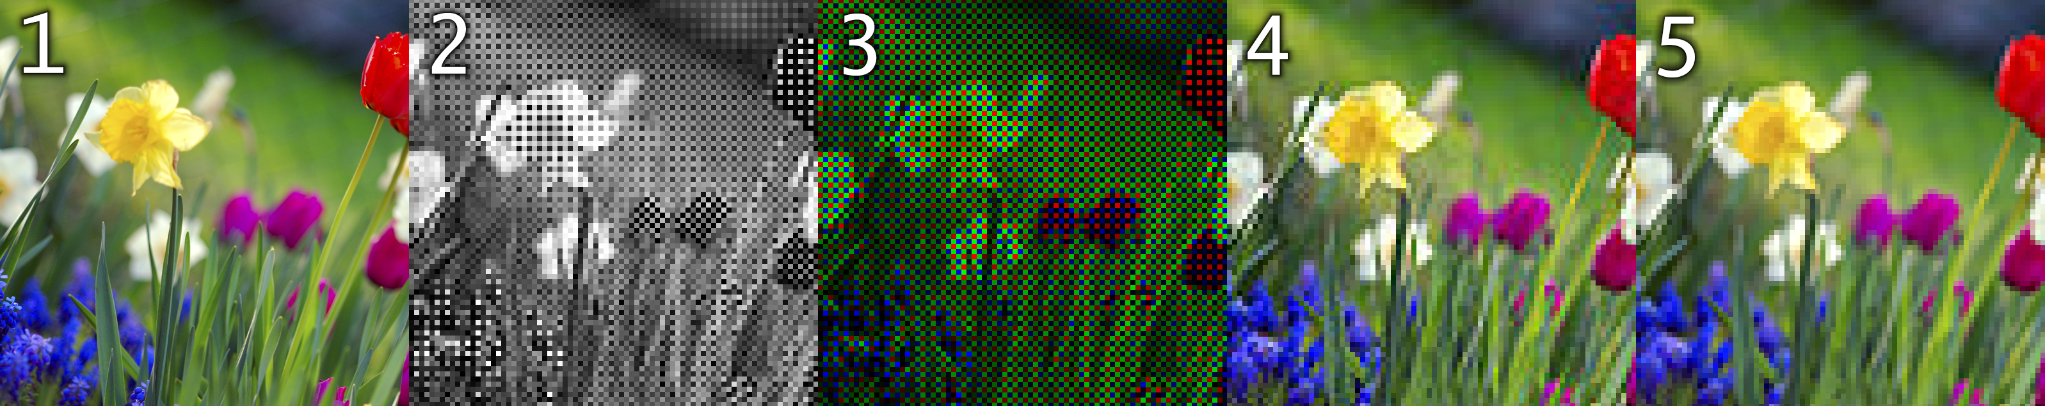
\includegraphics[width=\textwidth]{figures/horizontal_flowers.png}}{Demosaic process}
    \caption{Demosaic process \cite{demosaic}.}
    \label{fig:demosaic}
\end{figure}

\subsection{Colour Correction}
 \label{ss:cc}
Figures \ref{fig:xyz} and \ref{fig:d5100} demonstrate the significant differences in spectral sensitivities between the human eye and digital cameras, resulting in varying colour responses. Furthermore, the sensitivities can vary across different units of the same camera module \cite{walowit2019best}. In addition to colour inaccuracy, it also results in observer metamerism, where two cameras might see an object in differing colours while appearing the same for a human.

A colour correction matrix (CCM) is typically applied to the input image to account for the differences. The simplest way is to derive a 3x3 matrix by regression from camera responses to known XYZ responses for a standard observer. Like white balancing, this matrix is unique to each illuminant as white balancing only guarantees that neutral colours are mapped correctly \cite[1]{cheng2015beyond}. Furthermore, we can directly transform the input values to the desired output space, such as sRGB, with CCMs. This step is also often known as colour space transformation (CST).

Figure \ref{fig:cc} showcases the effect of colour correction, following a similar simulation process as in figure \ref{fig:wb}. On the left, we see the result of treating raw camera RGB values as sRGB values, resulting in an image with dull colours. On the right, colour correction has been performed to transfer the image from camera RGB to sRGB colour space, with the colours now being more saturated and vibrant.


\begin{figure}
    \centering
    \pdftooltip{
\includegraphics[width=\textwidth]{figures/cc.png}}{cc}
    \caption{Scene before and after applying Colour Correction, both with sRGB gamma applied. Image from Foster 2002 dataset \cite{foster:2002}. }
    \label{fig:cc}
\end{figure}


\subsection{Gamma}


Finally, the image has to be saved for storage. At this stage, the image is likely still in linear colour space, such as linear sRGB, and has to be transformed through a non-linear inverse gamma function to compensate for the monitor gamma \cite{4050037}. The gamma function is often modelled as follows:

\begin{equation}
V_{\text{out}} = V_{\text{in}}^\gamma,
\end{equation}

where $V_{\text{out}}$ is the output voltage after applying the gamma function, $V_{\text{in}}$ is the input voltage and $\gamma$ is the so-called decoding gamma. The camera pipeline thus applies the reciprocal gamma $V_{\text{in}}^{\frac{1}{\gamma}}$ at encoding phase. The effect of applying sRGB gamma to a set of greyscale values from black to white is displayed in Figure \ref{fig:gamma}. In the case of linear encoding, the gamma function is identity, so the output scales linearly with the scene's brightness. For sRGB encoding, the change from black to lighter greys is much more gradual and accurately represents how a human eye would perceive tones with a linear change in brightness.

\begin{figure}
    \centering
    \pdftooltip{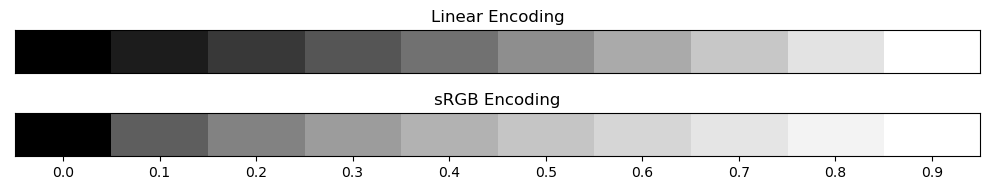
\includegraphics[width=\textwidth]{figures/gamma.png}}{gamma}
    \caption{Linear vs sRGB ($\approx 2.2$) Gamma Encoding.}
    \label{fig:gamma}
\end{figure}

Typically, the gamma is roughly $2.2$ to comply with colour spaces such as sRGB \cite{sRGB}. Inverse gamma was initially applied in images to compensate for non-linearities in CRT monitors. Still, it has also been found to closely simulate the human perception of brightness, which more accurately senses differences in darker tones. The input range becomes linear again when gamma decoding is performed on the monitor. When the image is viewed, the human eye performs its correction again, resulting in a similar perceived depth as stored.

\subsection{Post-processing}

In this phase, the process varies among manufacturers, focusing more on enhancing the image's visual appeal and ensuring it meets the intended output specifications. At this stage, the objective shifts from faithfully recreating the original scene to crafting an image representing an ideal version of what was observed.

Typical algorithms employed at this stage enhance the colours, for instance, by making them look more saturated and removing artefacts such as noise from the image. Sharpness is typically preferred, so an additional edge sharpening step is often performed  \cite[40-41]{Ramanath} \cite{4050037}.

Before display, the image is often compressed to save space. Some compression algorithms might discard information from the image that is not perceptually important to the viewer. Hence, they are often called lossy algorithms and convert the image into colour space with less correlation and detail across channels. Typical encoding formats encountered these days are some variants of JPEG \cite{JPEG} and PNG \cite{PNG}.


